\documentclass[a4paper]{article}
\usepackage[utf8]{inputenc}
\usepackage{amsmath}
\usepackage{amsfonts}
\usepackage{amssymb}
\setlength{\parindent}{0in}
\usepackage{fancyhdr}
\usepackage{graphicx}
\usepackage[margin=.8in]{geometry}

\begin{document}

\pagestyle{fancy}
\rhead{David Nápravník - přezdívka ":)" - v.3}

\setcounter{section}{1}
\section{du}
\subsection{}
Mejme uplny bipartitni graf velikosti $n,n$ kde na jedne strane jsou indexy policek a
na druhe cisla ktera do nich budeme dosazovat.\\
Dale mejme latinsky obdelnik rozmeru $r*n$ kde $n>r$.\\
V bipartitnim grafu odeberme hrany jenz jiz jsou soucasti latinskeho obdelniku.\\
\textit{Pozorovani:} kazda hrana je stupne $n-r$\\
Tudiz radku $r+1$ pak bude na pozici kazdeho indexu mozno priradit rozdilne cislo.
Dle hran ktere vedou z daneho vrcholu v grafu do vrcholu s cislem. 


\subsection{}
\begin{itemize}
\item neplati\\
Dukaz obrazkem, kde mame tri body jez nejsou na kruznici.\\
\begin{center}
    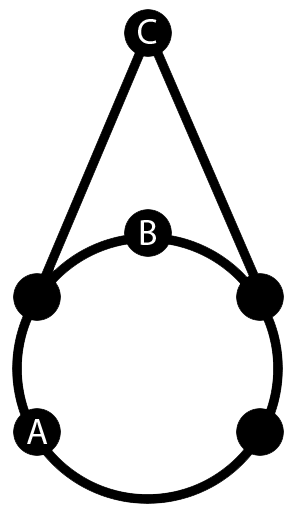
\includegraphics[scale=0.3]{notBipartial.png}    
\end{center}

\item plati\\
Takovy vrchol musi existovat, nebot pro "zniceni souvislosti" grafu musime
odebrat 3 vrcholi, takze muzeme odebrat vrchol $z$ a graf musi byt vrcholove
2-souvisly a tudiz obsahuje kruznici. Neboli kruznici na ktere nelezel bod $z$.

\item neplati\\
specificky nebude platit pro graf "motylka"\\
motylek: graf o dvou n-kompletnich grafech spojenych pres jediny vrchol.
Takovy graf bude n-hranove souvisly, ale pouze 1 vrcholove.
Tudiz pro $k>1$ neexistuje dostatecne velke $l$, tudiz tvrzeni neplati.
\end{itemize}


\subsection{}
\textbf{puze pro k=1}, jedine graf kde kazda hrana obsahuje maximalne jeden
vrchol splni Hallovu podminku. Nebot pro $k>1$ existuje hypergraf takovy, ze
mame vice hran nez vrcholu.


\subsection{}
Kostra spojuje kazde dva vrcholy prave jednou cestou.
Dalsi disjunktni kostra nam prida disjunktni cestu mezi kazdymi dvemi vrcholi.
Tudiz kolik disjunktnich koster graf ma,
tolik disjunktnich cest existuje mezi kazdymi dvemi vrcholy.
Z cehoz plyne ze takovy graf bude \textbf{hranove k-souvisly}.
\\
O vrcholove souvislosti nam to nic nerekne, nebot muze nastat graf typu motylek
viz vise. A takovy graf bude tedy pouze \textbf{vrcholove 1-souvisly}.


\end{document}